This lecture studies some of the key assumptions we have previously imposed on the auction to derive various result, and what happens if these assumptions are not upheld.

\begin{figure}
  \centering
  \caption{Assumptions required for revenue equivalence}
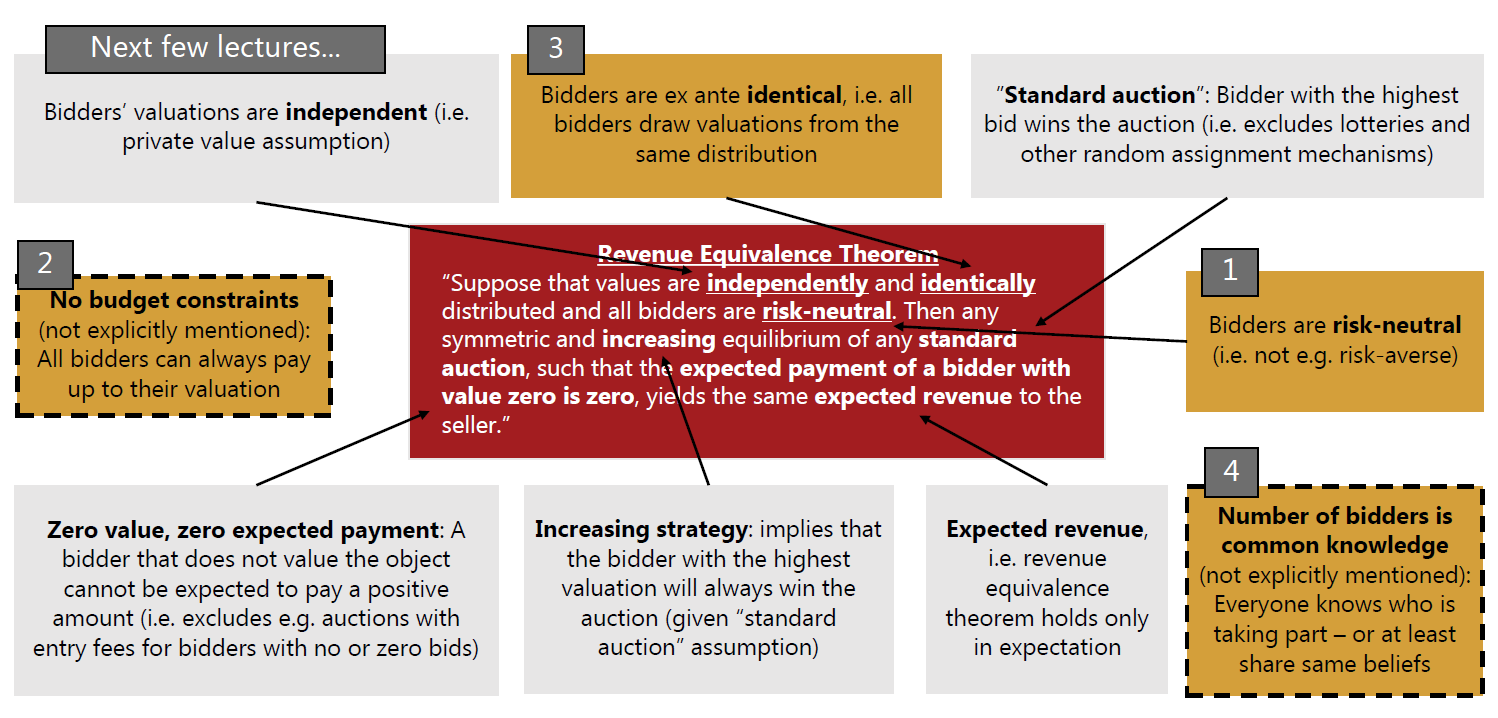
\includegraphics[width=0.8\textwidth]{figures/assumptions.PNG}
\end{figure}

\subsection{Risk neutrality}
So far we have assumed bidders to be risk neutral, so that their decision does not put any additional weight to winning the auction appart from the pure value of the item. When this assumption holds, agents can maximize expected profits (instead of expected utility) simplifying their decisions. Mathematically we would say risk-neutral bidders have quasi-linear preferences such that $u(\cdot): \mathbb{R}_+ \rightarrow \mathbb{R}$ has $u'>0, u''=0$.

Risk averse bidders on the other hand have concave utility.

\subsubsection{Risk aversion in the second price auction}
In the second price auction risk preferences does \textit{not} play any role in deriving the symmetric equilibrium. This is in essence because the equilibrium is ex-post optimal in the seond price auction, meaning there is no potential for regretting ones bid.

\subsubsection{Risk aversion in the first price auction}
In the second price auction risk preferences play a role, in particular we solve for the equilibrium by assuming the bidder wants to maximize expected profits. In the case of risk aversion the bidder would want to maximize expected profits while balancing the risk of not winning the auction. every time the risk averse bidder lowers his bid he not only reduces the probability of winning, but also incurs a risk-cost from the reduced change of winning.

oppositely risk loving bidders will shade even more than risk neutral ones, because they assign a positive value to the risk of not winning the auction.
\begin{align*}
  &\textrm{Gain from winning } \underset{balance}{-} \textrm{ P(win)} && \textrm{ Risk neutral} \\
  & \textrm{Gain from winning }  \underset{balance}{-} \textrm{ P(win)} + \textrm{price of loosing} && \textrm{non-neutral}
\end{align*}

In conclusion risk averse bidders shade less than risk-neutral bidders in the first price format.
\\ \\
\subsubsection{Revenues and efficiency under risk aversion}
Risk averse bidders also affect the revenue equivalence of first and second price auctions.
\begin{proposition}{Revenue equivalence under risk aversion:} Risk averse bidders with the same utility function and symmetric independent private values give a higher expected revenue in first price auctions than in second price auctions.
\end{proposition}
\begin{proof}
  Risk profiles does not affect the second price auction, but cause all bidders to shade less in the first price format. Thus revenues cannot be equivalent, and must be higher in the first price auction.
\end{proof}
Note that as long as all bidders are equally risk averse, both auction formats are still efficient.

\subsection{Budget constraints}
So far we've assumed that bidders can always bid their intended bid, but often this is not the case (think the case with entrepreneurs in Copenhagen).

\subsubsection{Budget constraints in the second price auction}
In second price auctions the optimal strategy under a budget constraint becomes to bid ones valuation if possible, and otherwise the full budget, i.e. $\min\{x,w\}$ where $w$ is the budget limit. The proof of this is completely parallel to the one without a budget constraint, execpt now we need to account for the cases where $x>w$ where one could bid below $w$ and risk loosing out on a win, or bid above $w$ and risk winning at a price higher than affordable (which we assume gives a profit of 0).

\subsubsection{Budget constraints in the first price auction}
In first price auctions once again the bidding strategy is only affects when the budget constraints become binding, so $\beta^I(x,w)=\min\{\beta^I(x), w\}$. The reasoning is that when $\beta(x)<w$ the logic without budget constraints applies, while at $\beta(x)>w$ it is a weakly dominated strategy to bid above $w$ as winning in this case gives 0 profit.

\subsubsection{Revenues and efficiency under budget constraints}
With budget constraints expected revenues are higher in first price auctions than in second price auction. The reason is that in first price auctions the bidders shade, meaning less of them will be budget constrained. Since revenues are identical without budget constraints this implies a larger decrease in revenue in second price auctions.
\\ \\
Clearly budget constraints can lead to inefficiency - as the bidder with the highest valuation might be budget constrained at a very small budget. If all bidders face the same budget, auctions can still be inefficient as the auctioneer will have no way to determine the right winner if bids are at the constraints limit $w$.


\subsection{Asymmetric distributions}
So far our baseline assumption has been that all individuals have identical valuation distributions, i.e. bidders are ex ante identical

\subsubsection{Asymmetric bidders in the second price auction}
In the second price auction bidders valuation distributions are not important for deriving the equilibrium strategies.

\subsubsection{Asymmetric bidders in the first price auction}
In the first price auction we use the assumption of symmetric bidders in out definition of $G(\cdot)$, we will consider a special case of asymmetry, namely one with two bidders with different distributions of $x$, so
\begin{equation}
 X_1 \sim F_1:[0,\omega_1] \qquad X_2 \sim F_2:[0,\omega_2]
\end{equation}
where bidders follow $\beta_1, \beta_2$ and we impose that $\beta_1(0)=\beta_2(0)=0$ while $\beta_1(\omega_1)=\beta_2(\omega_2)=\bar(b)$ i.e. that both bidders submit bids on the same range. We then consider a special case of asymmetry where $F_2$ stochastically dominates $F_1$ so $\forall x \in(0, \omega_2):F_1(x)\leq F_2(x)$ where $\omega_2 \leq \omega_1$ meaning the bidder with the largest range of valuations (bidder 1)'s probability of drawing at least $x$ is always larger than the probability that the weak bidder draws at least $x$.

In this case the weak bidder (bidder 2) will bid more aggressively than the strong bidder (bidder 1), that is $\beta_2(x)>\beta_1(x)$ for all $x$ in $[0, \omega_2]$. This is intuitively because the weak bidder realizes he is very unlikely to win, making it worth shading less, to increase the probability of winning.

\subsubsection{Revenue equivalence and efficiency under asymmetry}
In general we do not have revenue equivalence under the assymetric model, but which auction performs better depends on the concrete distributions of bidders valuations, meaning no general ranking of auction formats can be made. When distributions are uniform however, the expected revenue is higher in a first price auction than in the second price auction (see example 4.3, 4.4 in krishna).
\\ \\
With asymmetry the first price format can be inefficient, while the second price format will still be efficient. In the first price format the aggresiveness of the weak bidder implies there will be some cases where the weak bidder wins even though the strong bidder had drawn a higher valuation.


\subsection{Uncertain number of bidders}
So far we've assumed that the number of bidders is common knowledge but in many cases especially whn there are few potential bidders this might not be the case.

\subsubsection{Uncertain number of bidders in the second price auction}
The second price auction strategies is independent of the number of bidders. As a single opposing bidder is enough for the "bid your valuation" argument to hold.

\subsubsection{Uncertain number of bidders in the first price auction}
In the first price auction the number of bidders directly influence ones expectation of $Y_1$. In this case uncertainty on $N$ requires bidders to form beliefs about the true $N$ by guessing that $N=n$ with some probability. The bidding strategy then becomes an average of optimal bids under each possible $N$ weighted by the probability that it is the true $N$. This is of course assuming all bidders have the same beliefs over possible values of $N$, which might not be the case. In many cases it is likely that this density is asymmetric between bidders - imagine for example an oil drilling rights auction. In this case there might be 2-3 certain bidders, who have to guess if a new company will enter, while the new company can for certain know if they enter or not.

\subsection{Resale and efficiency}
One key concern in auction design is efficiency - i.e. selling to the bidder who wants the item the most. However one might argue that resale markets will always lead to efficient outcomes so auctioneers might as well maximize revenue regardless of the concerns for efficiency.
\\ \\
In the second price format we are almost always guaranteed efficiency, but under asymmetry the first price format is sometimes inefficient. It can be shown that this inefficiency is not easily cured by resale markets, as bidders will try to hide their true types as to not reveal it before the resale market. In this case the buyer who ends up with the item has no information about who actually has the highest valuation, and thus is no better of than in the first auction, and gives the possibility that no buyers really want the item on the resale market.
